% !Mode:: "TeX:UTF-8"
% !TEX program  = xelatex
% \section*{数据获取函数}\label{A:data}
% \Python{utils.py}{code/examples/utils.py}

% \section*{机器人物料表}


% \clearpage
\section*{部分零件机械设计图纸}

\begin{figure}[h!]
  \centering
  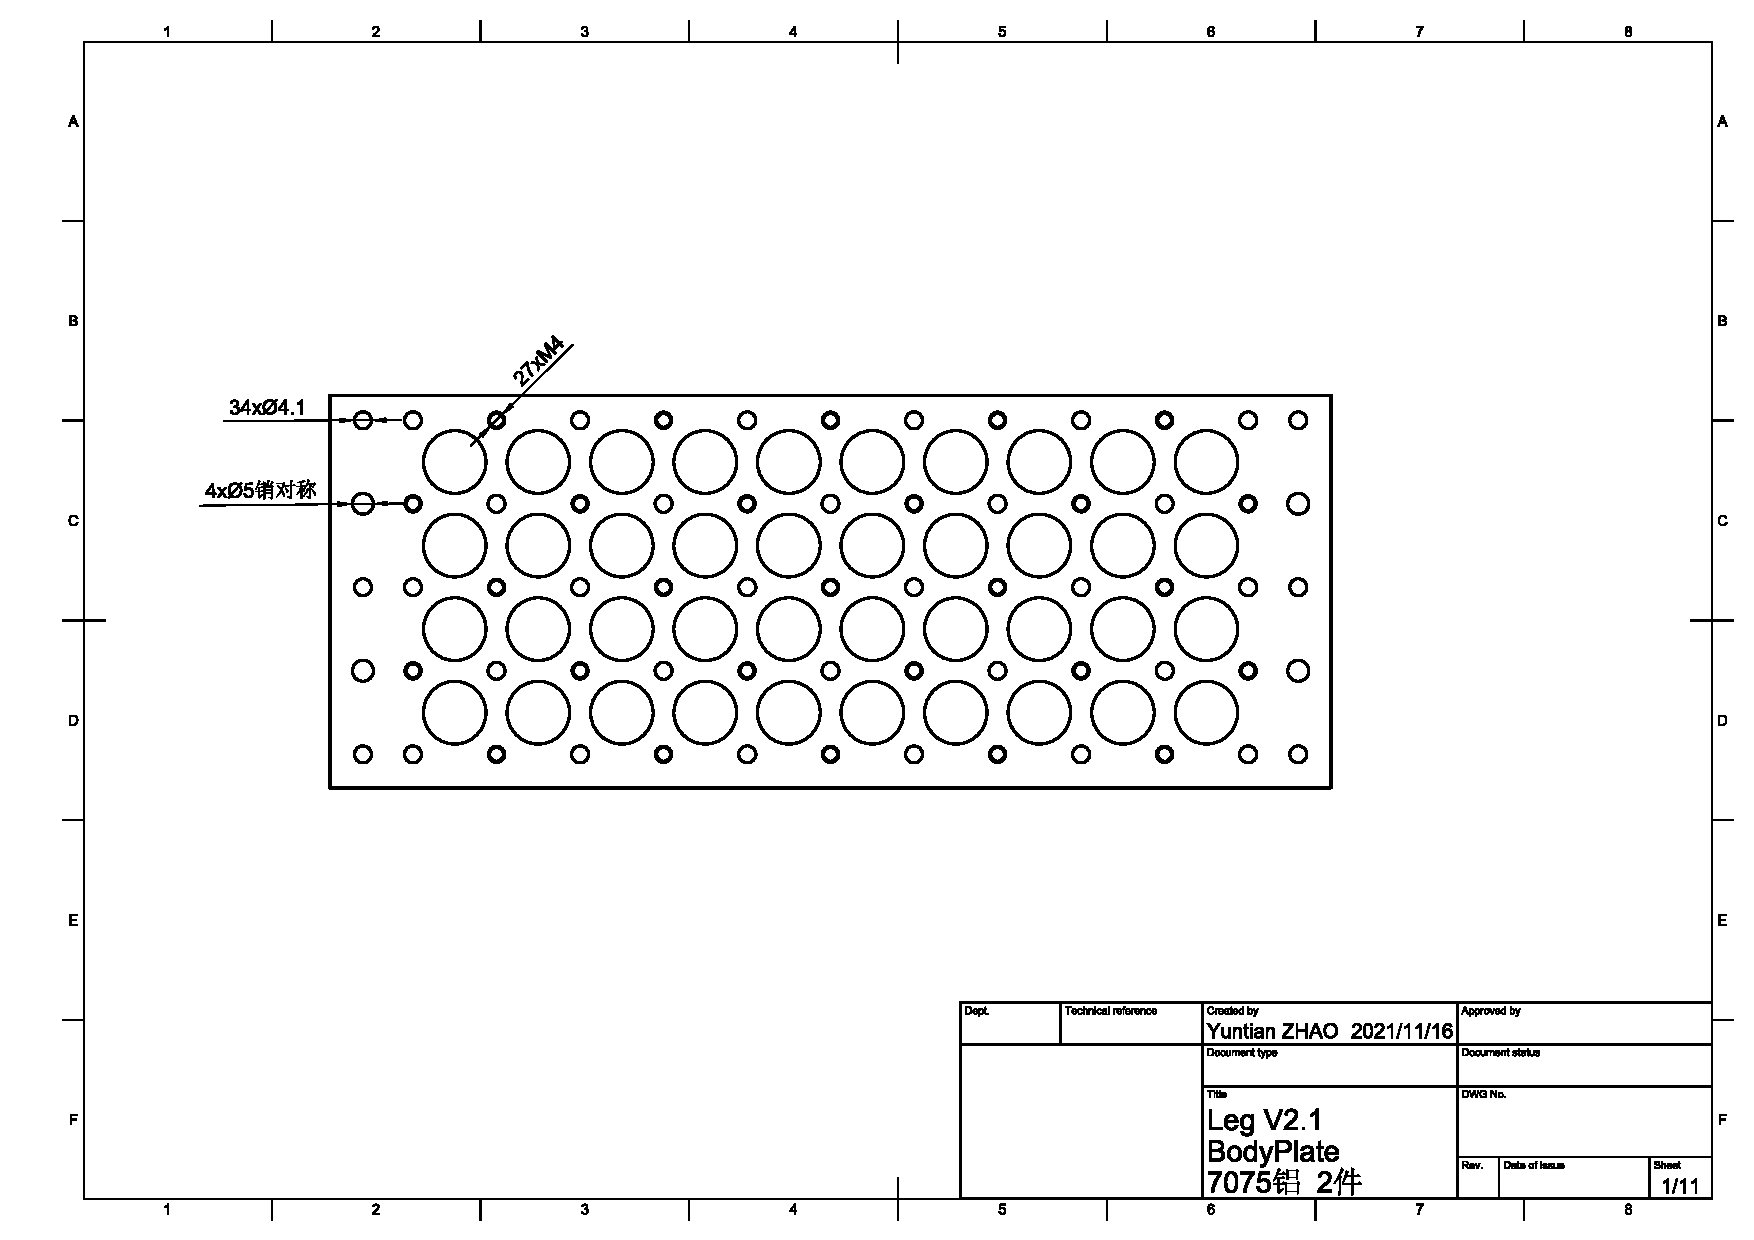
\includegraphics[width=1.4\linewidth, angle=90]{figures/appendix/dwg1.pdf}
   \vspace{6pt}
\end{figure}

\begin{figure}
  \centering
  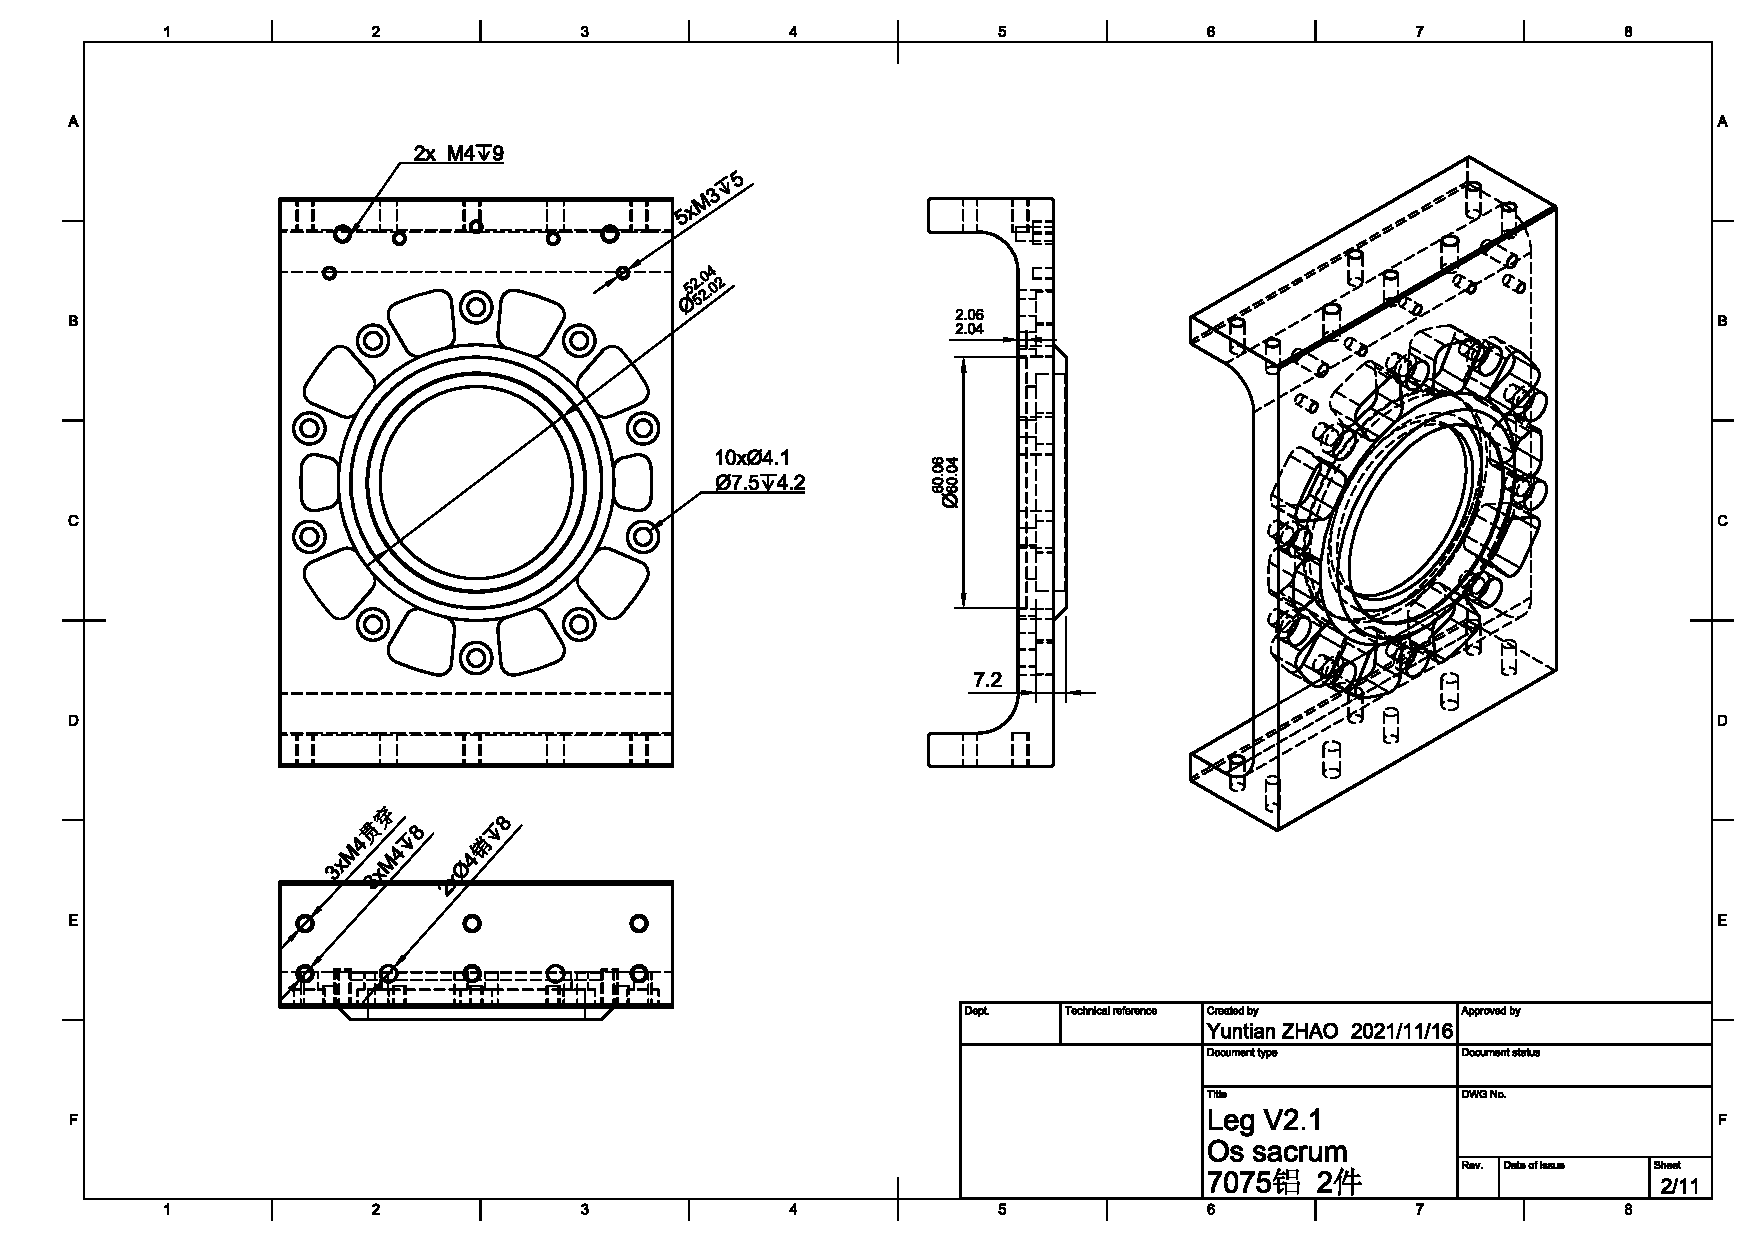
\includegraphics[width=1.4\linewidth, angle=90]{figures/appendix/dwg2.pdf}
   \vspace{6pt}
\end{figure}

\begin{figure}
  \centering
  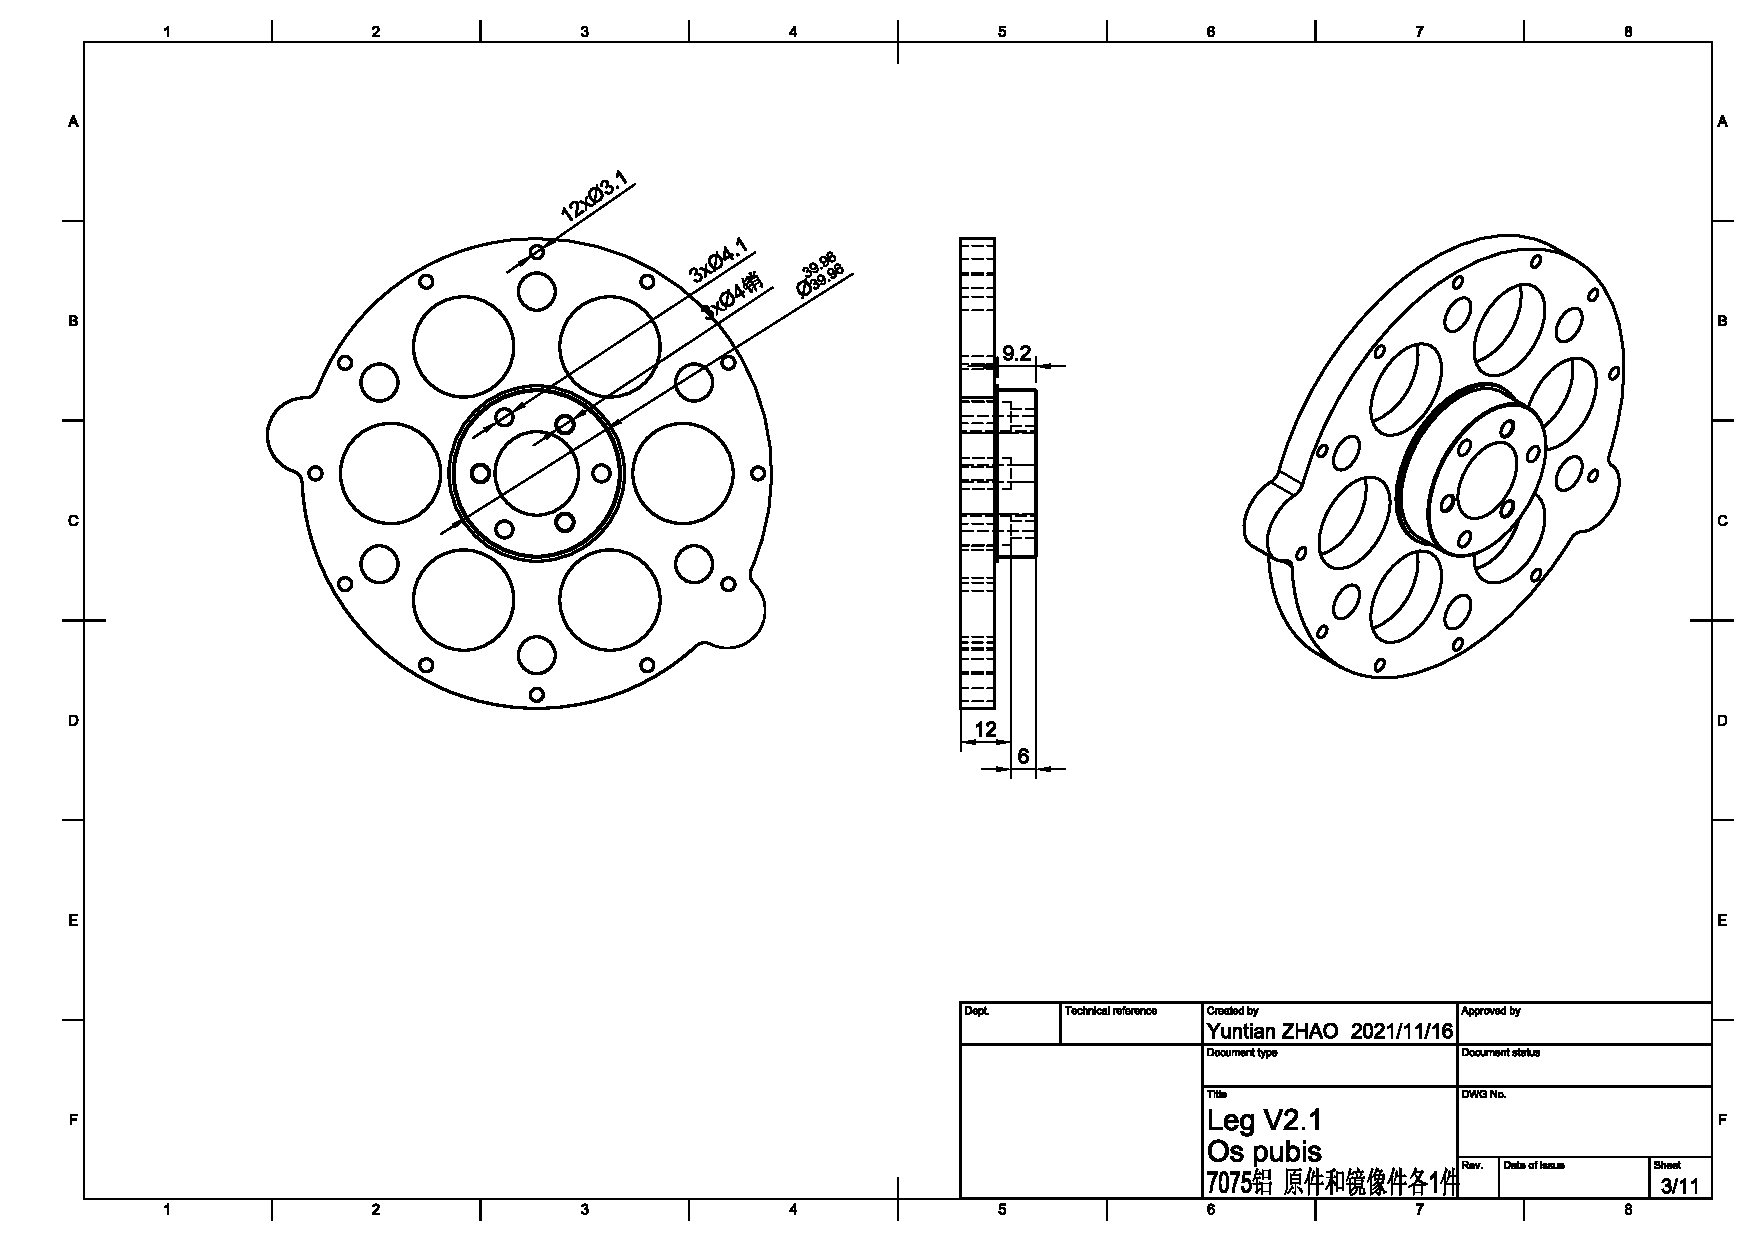
\includegraphics[width=1.4\linewidth, angle=90]{figures/appendix/dwg3.pdf}
   \vspace{6pt}
\end{figure}

\begin{figure}
  \centering
  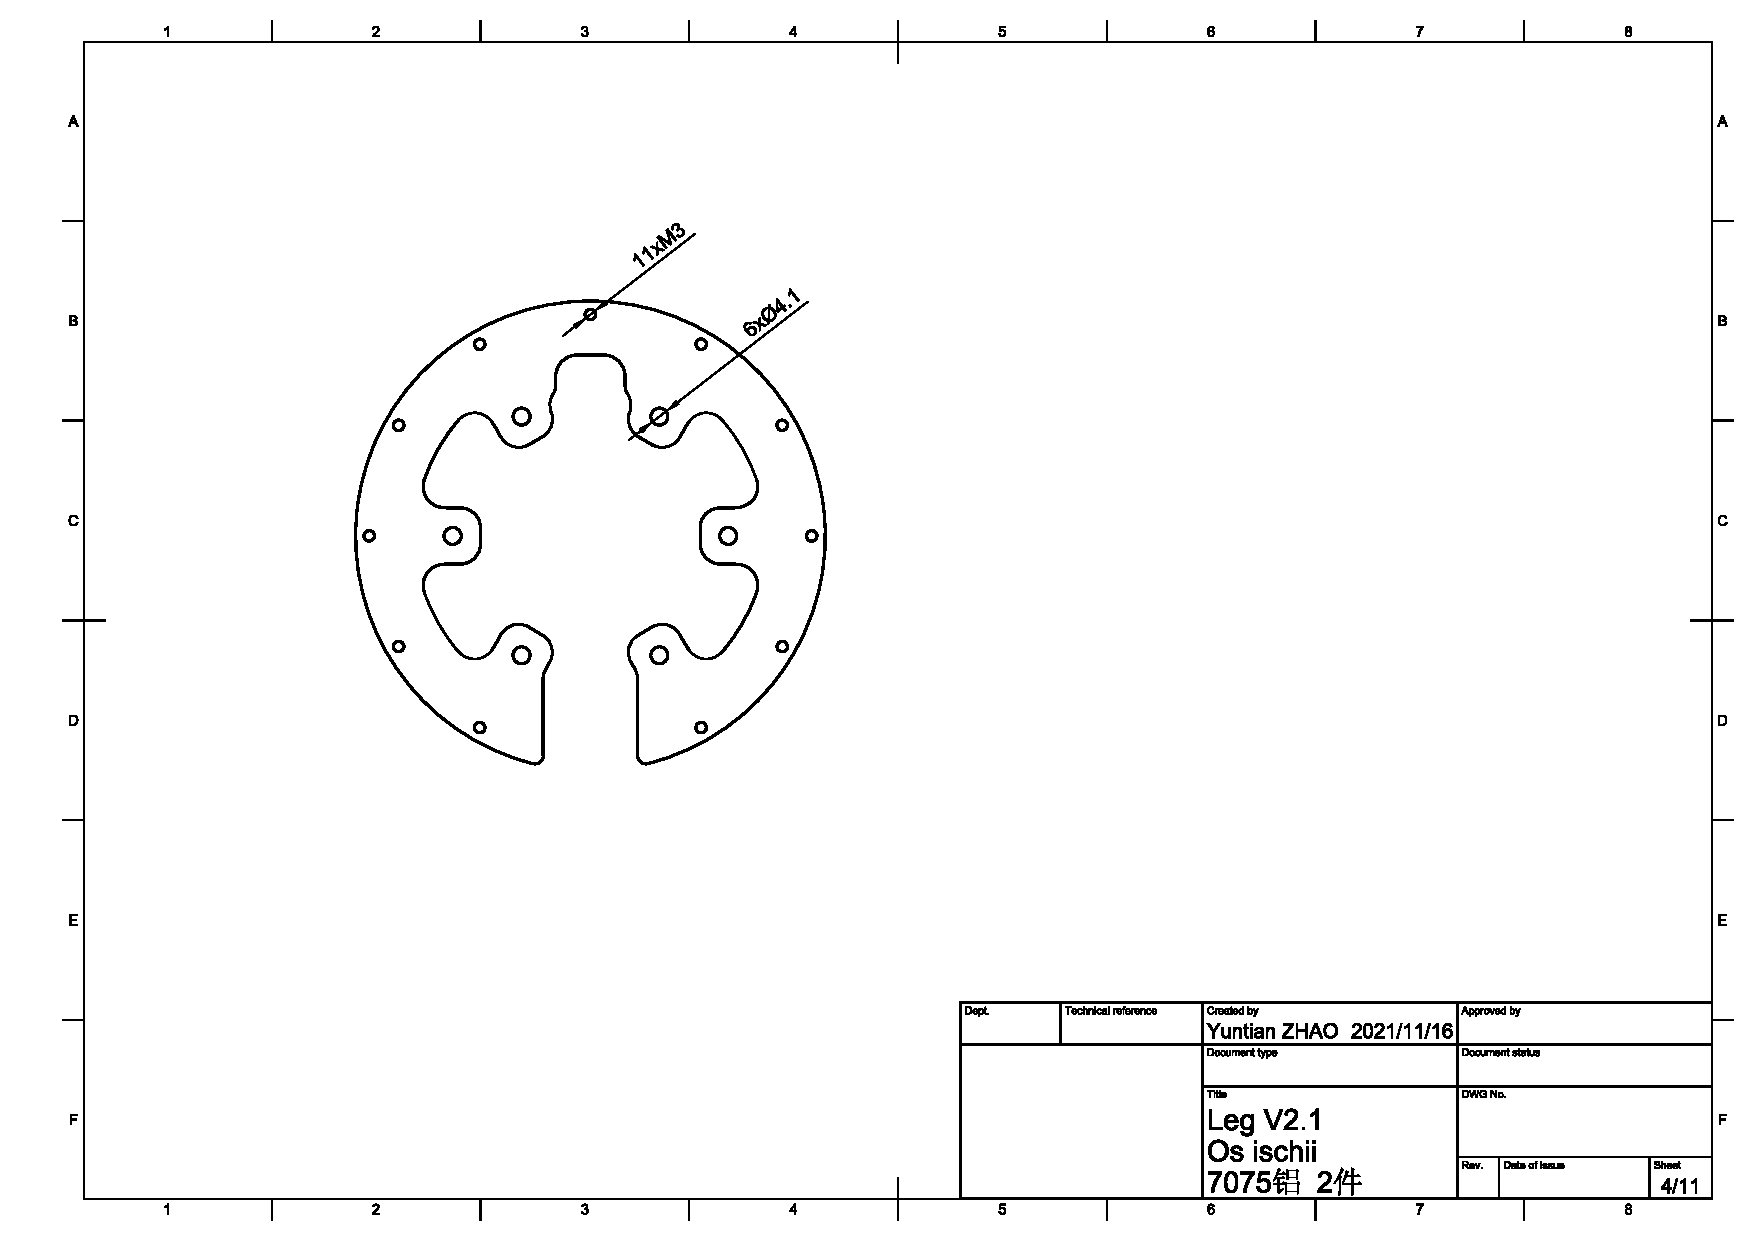
\includegraphics[width=1.4\linewidth, angle=90]{figures/appendix/dwg4.pdf}
   \vspace{6pt}
\end{figure}

\begin{figure}
  \centering
  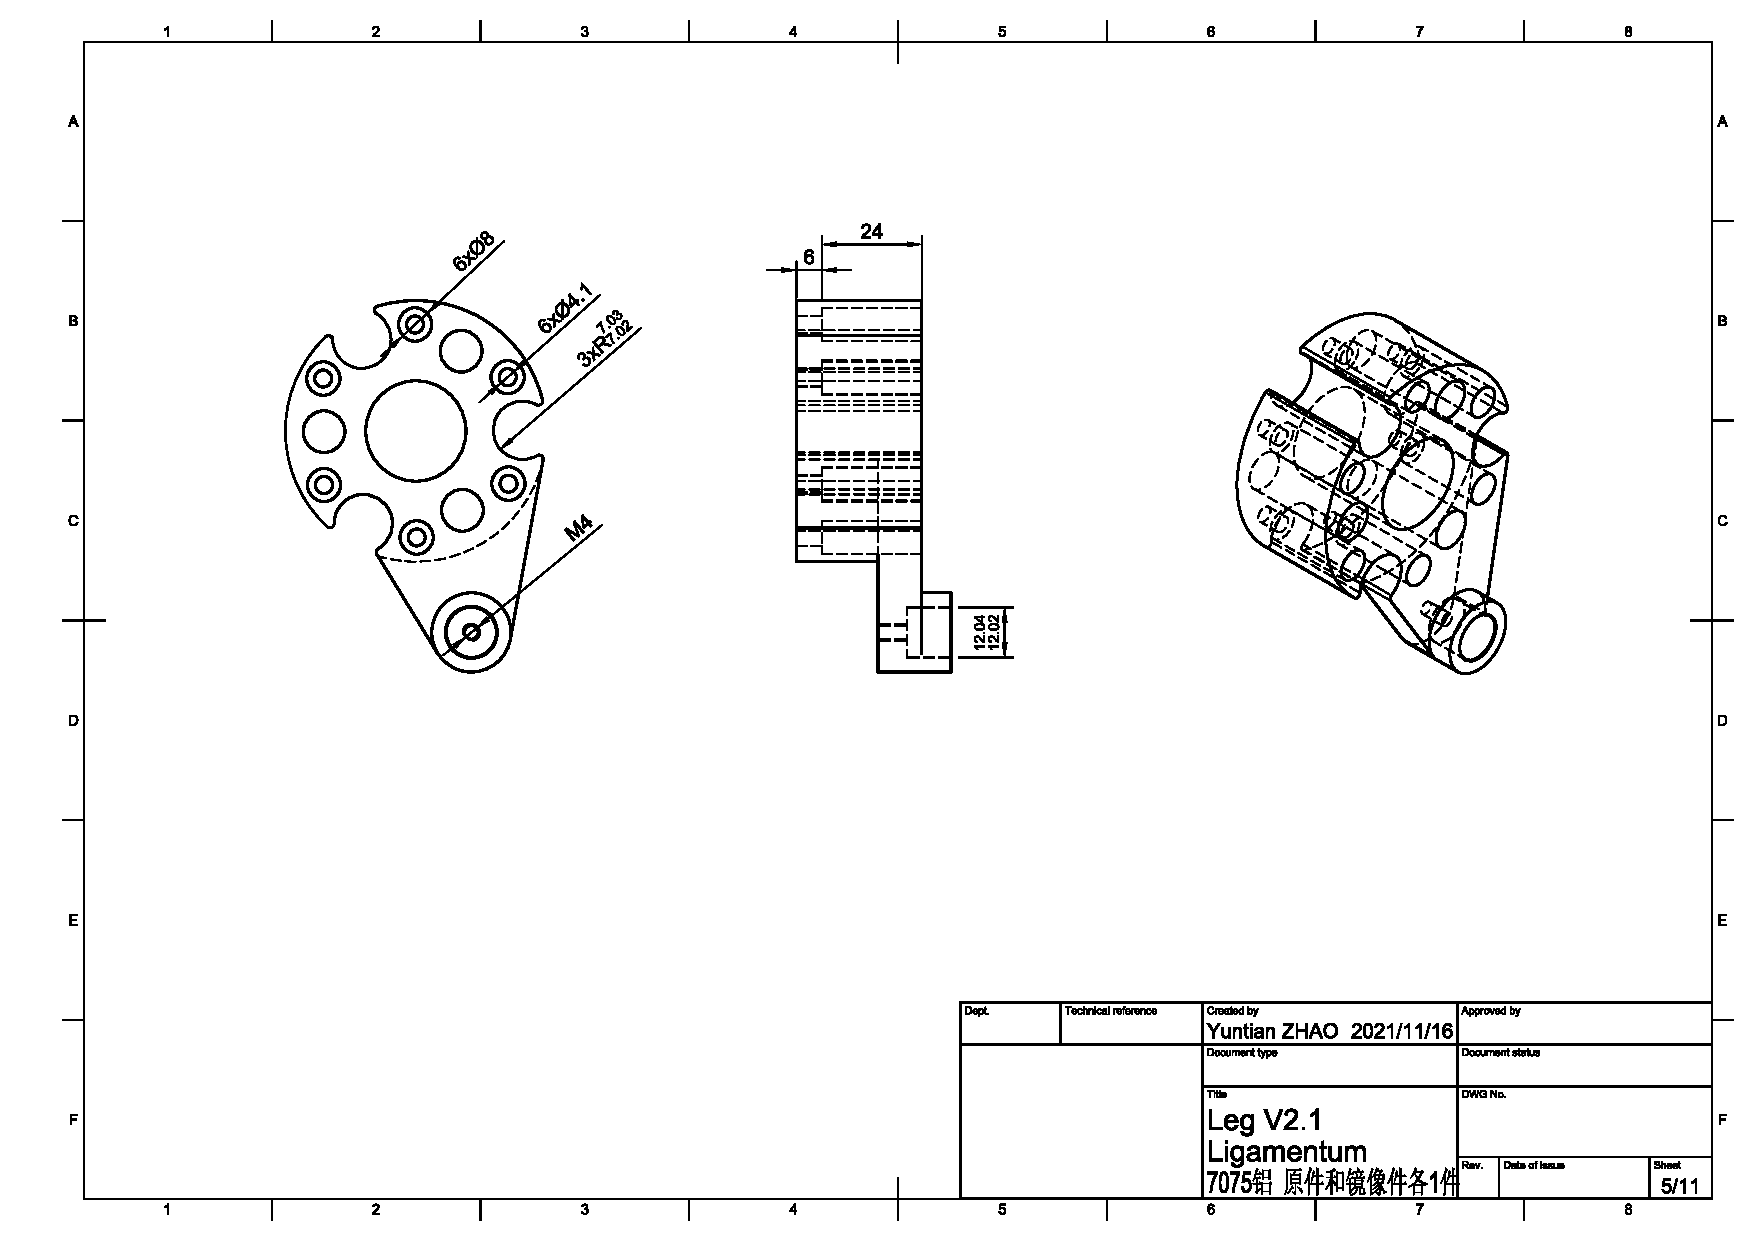
\includegraphics[width=1.4\linewidth, angle=90]{figures/appendix/dwg5.pdf}
   \vspace{6pt}
\end{figure}

\begin{figure}
  \centering
  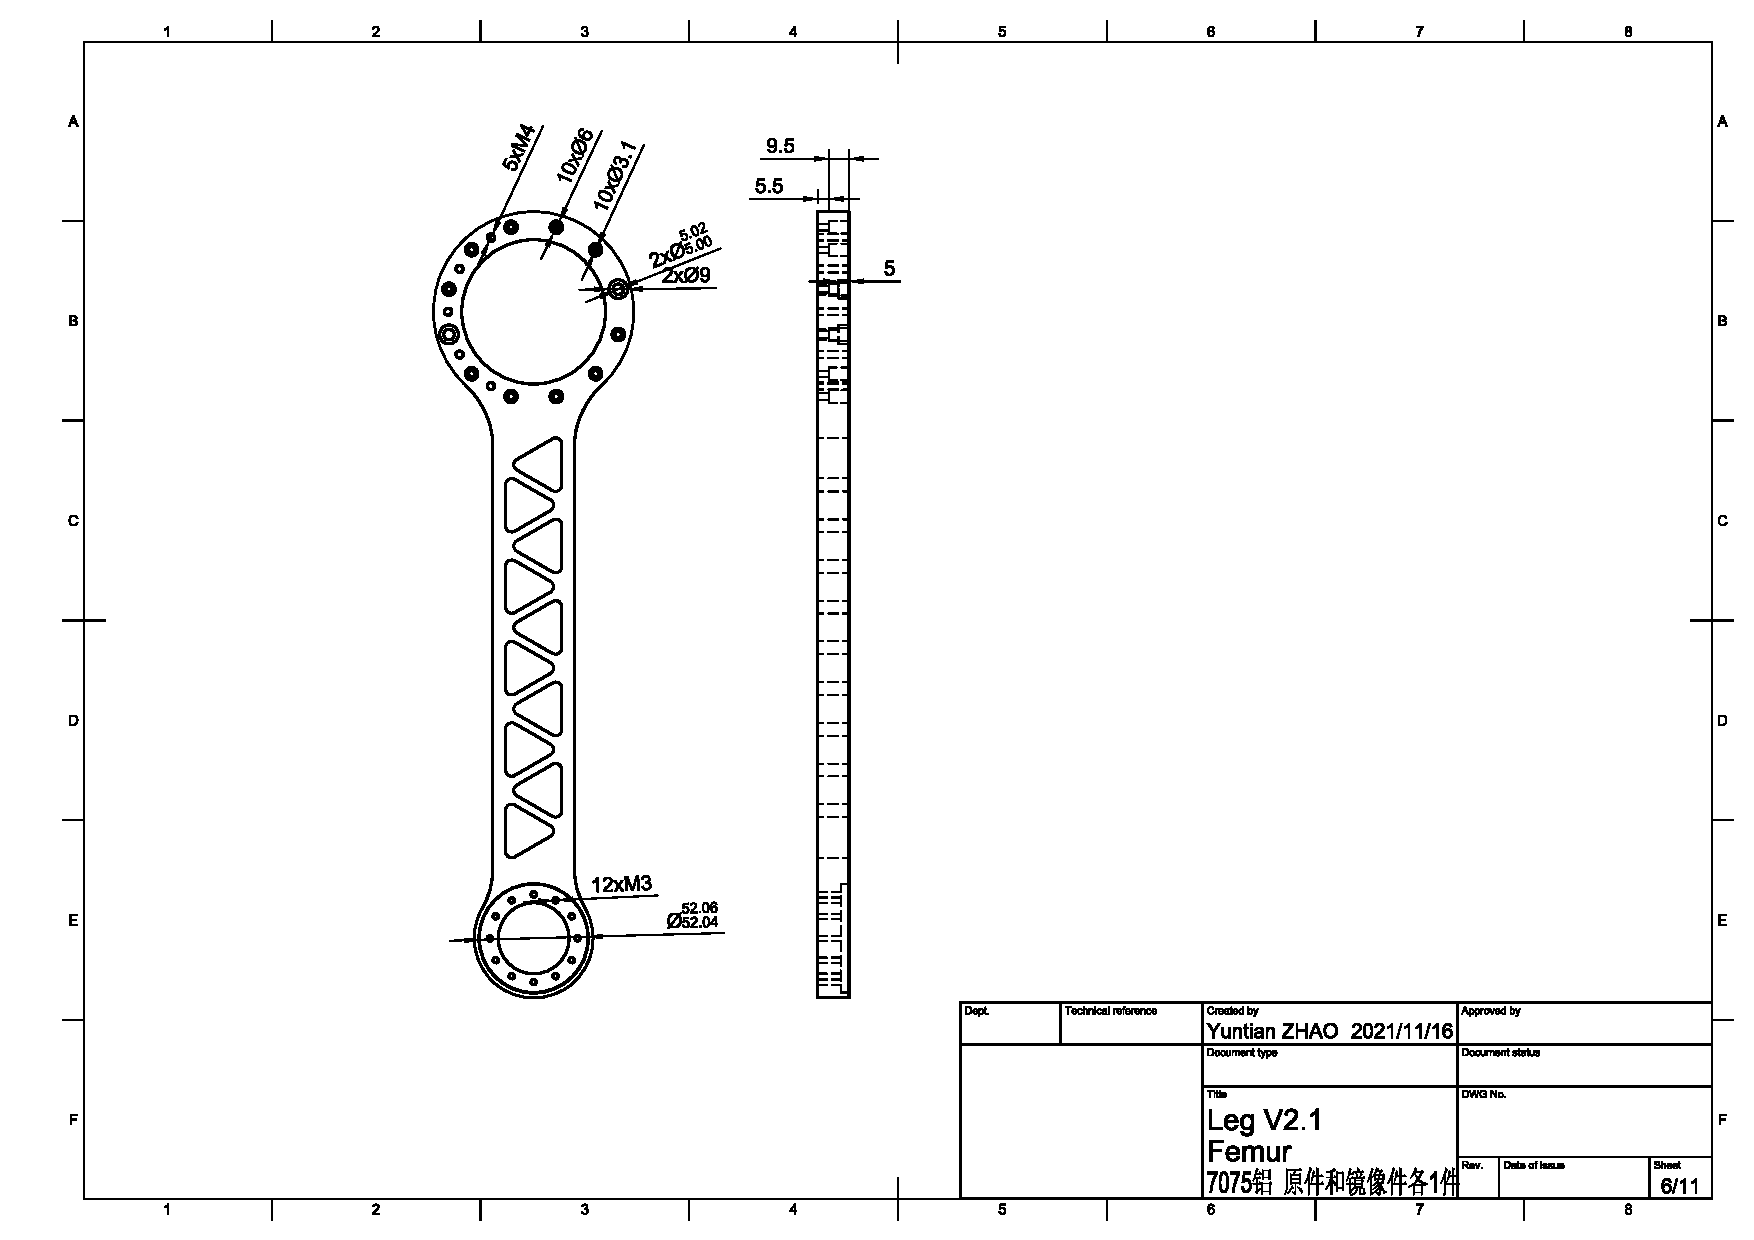
\includegraphics[width=1.4\linewidth, angle=90]{figures/appendix/dwg6.pdf}
   \vspace{6pt}
\end{figure}

\begin{figure}
  \centering
  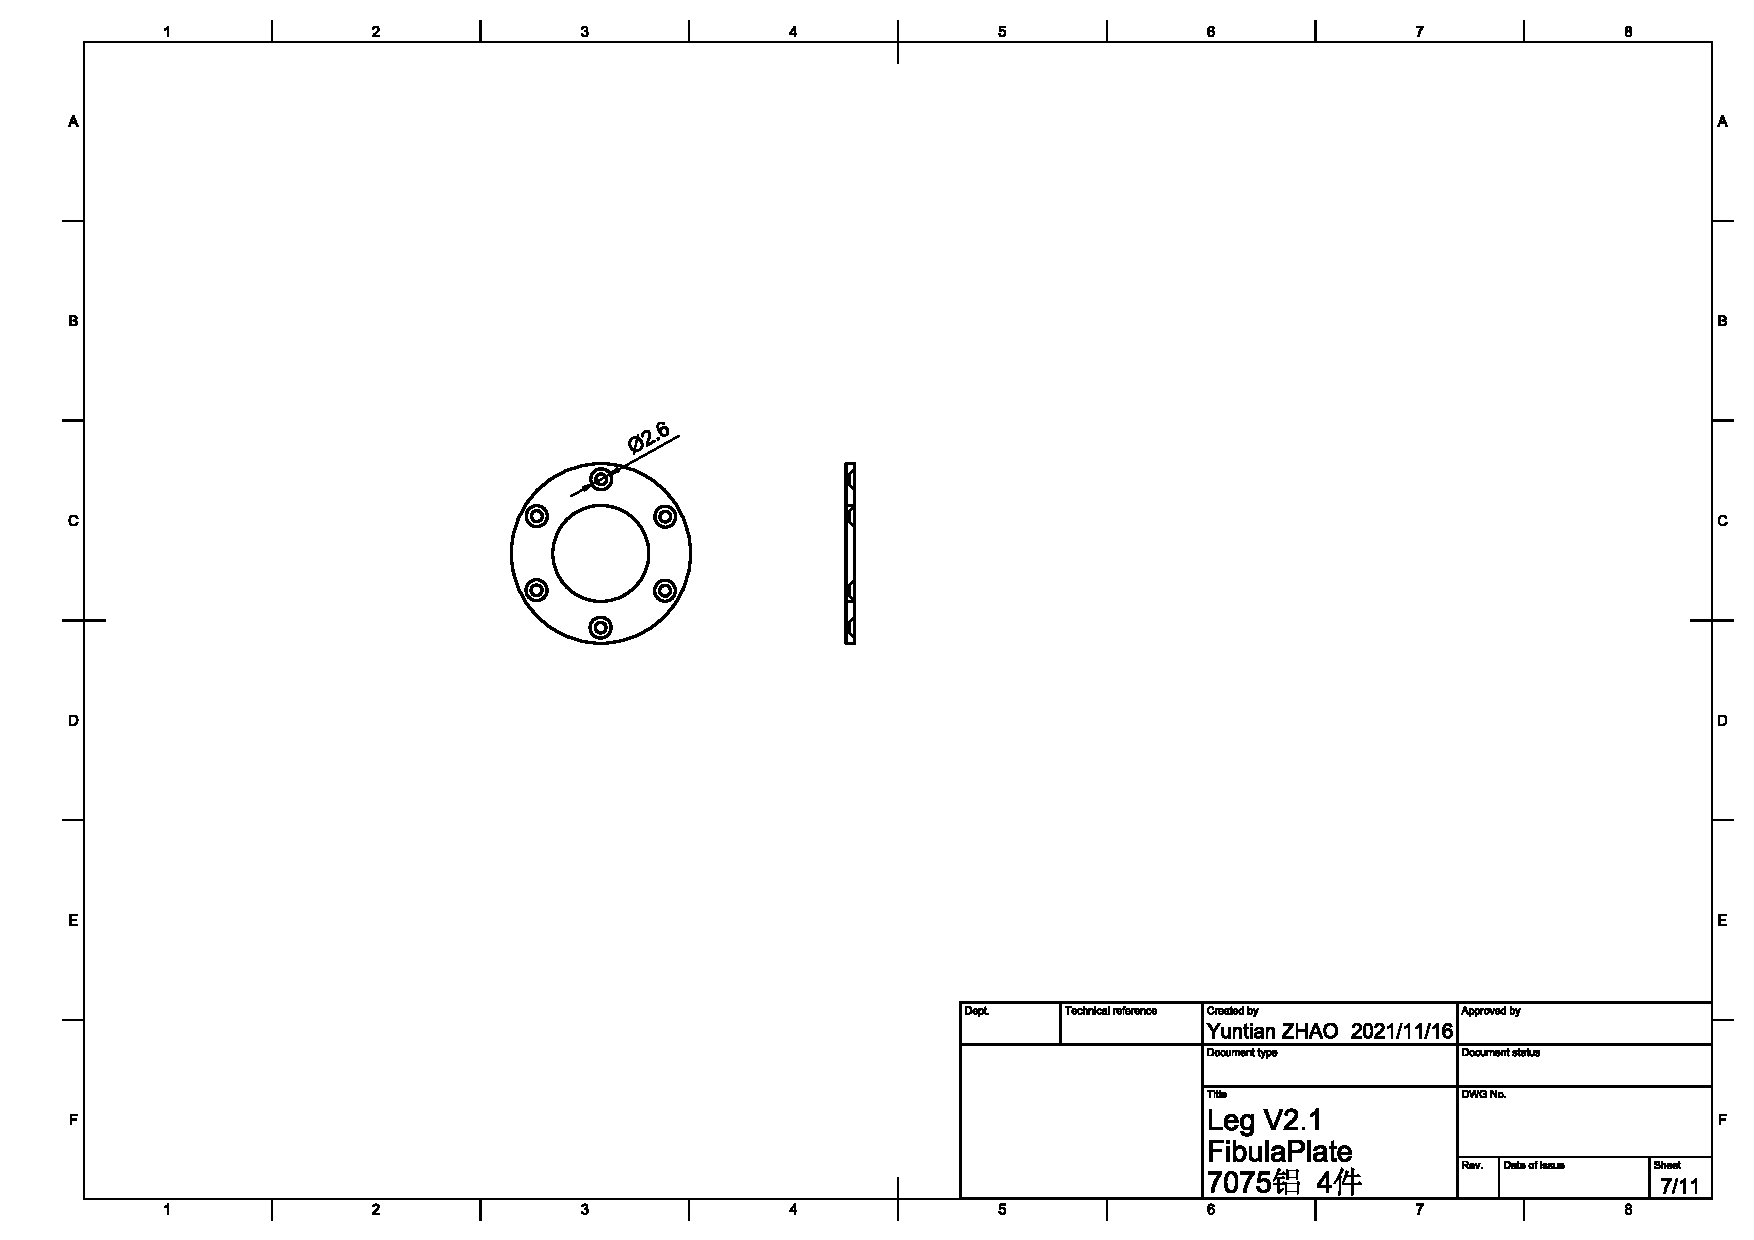
\includegraphics[width=1.4\linewidth, angle=90]{figures/appendix/dwg7.pdf}
   \vspace{6pt}
\end{figure}

\begin{figure}
  \centering
  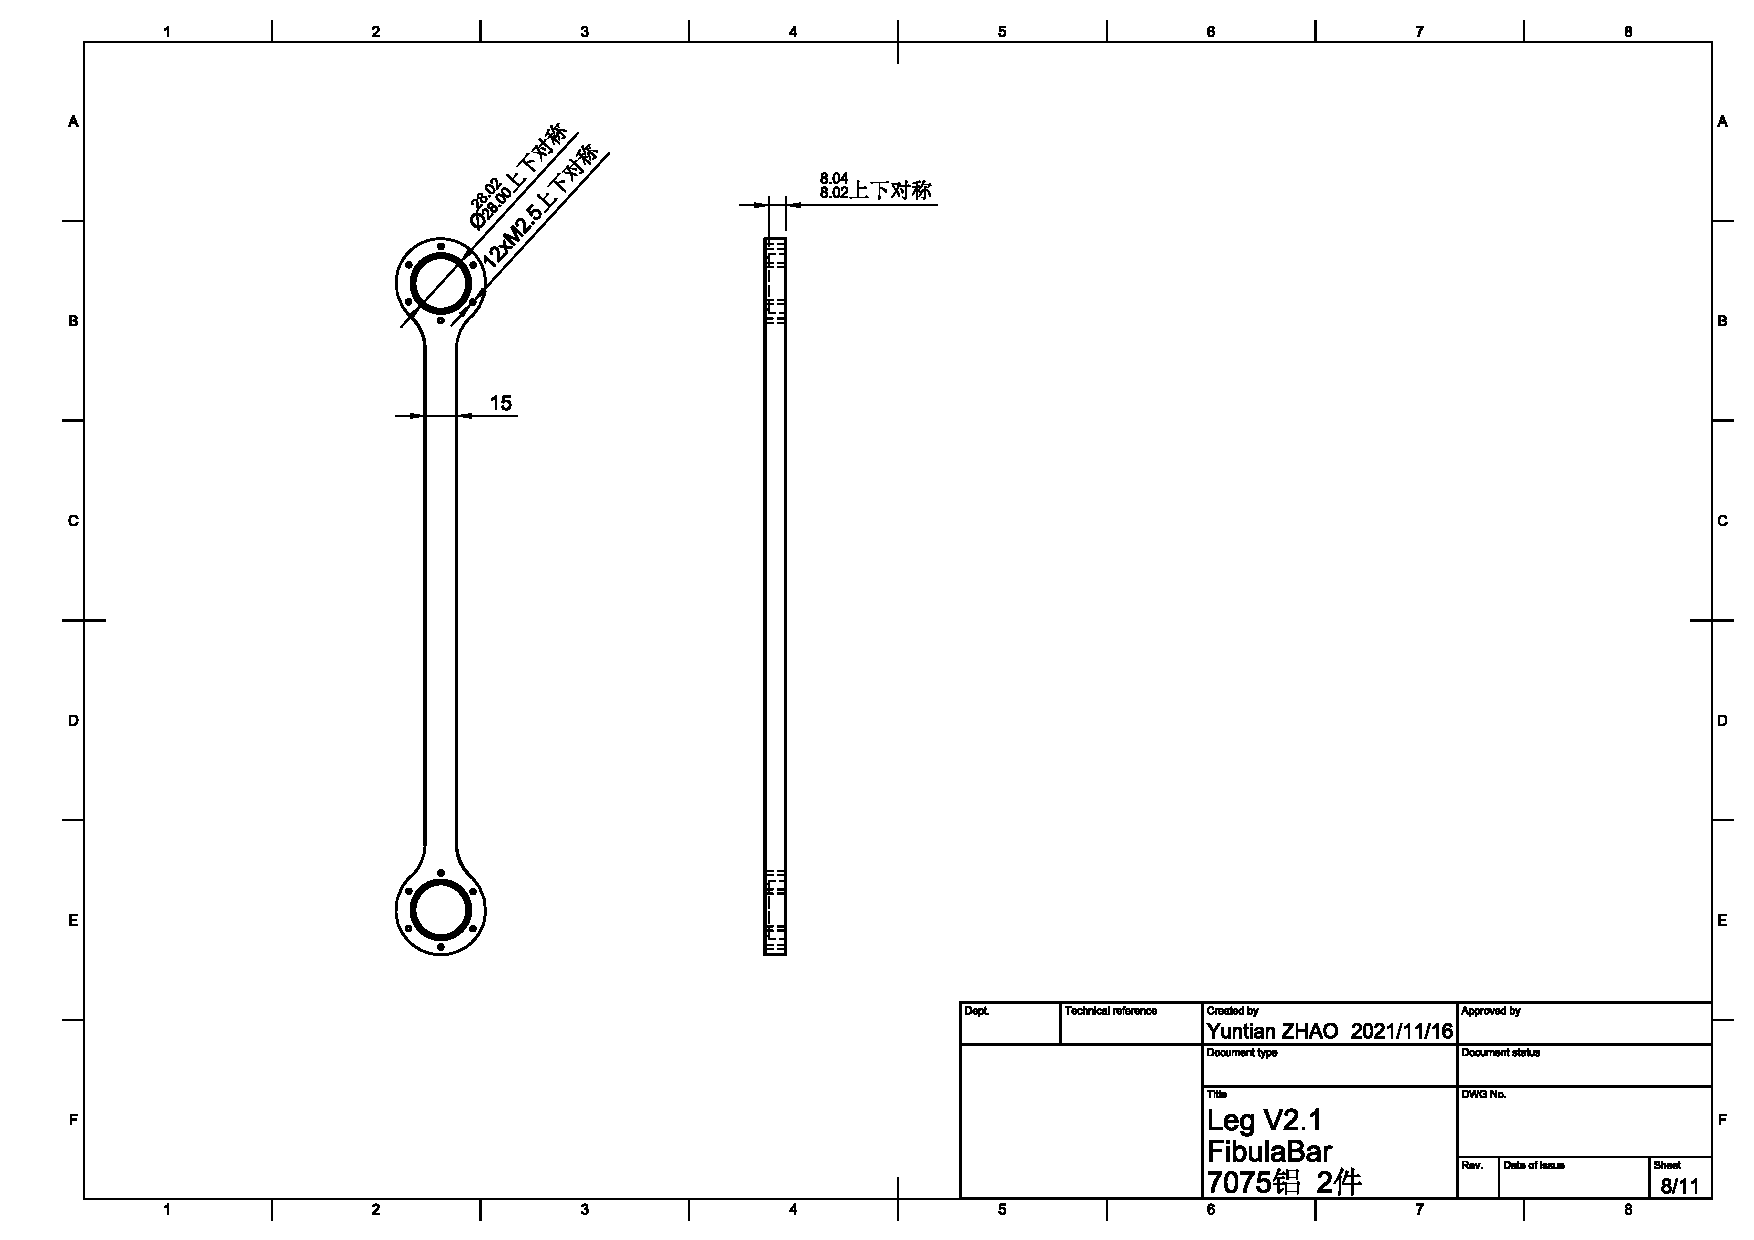
\includegraphics[width=1.4\linewidth, angle=90]{figures/appendix/dwg8.pdf}
   \vspace{6pt}
\end{figure}

\begin{figure}
  \centering
  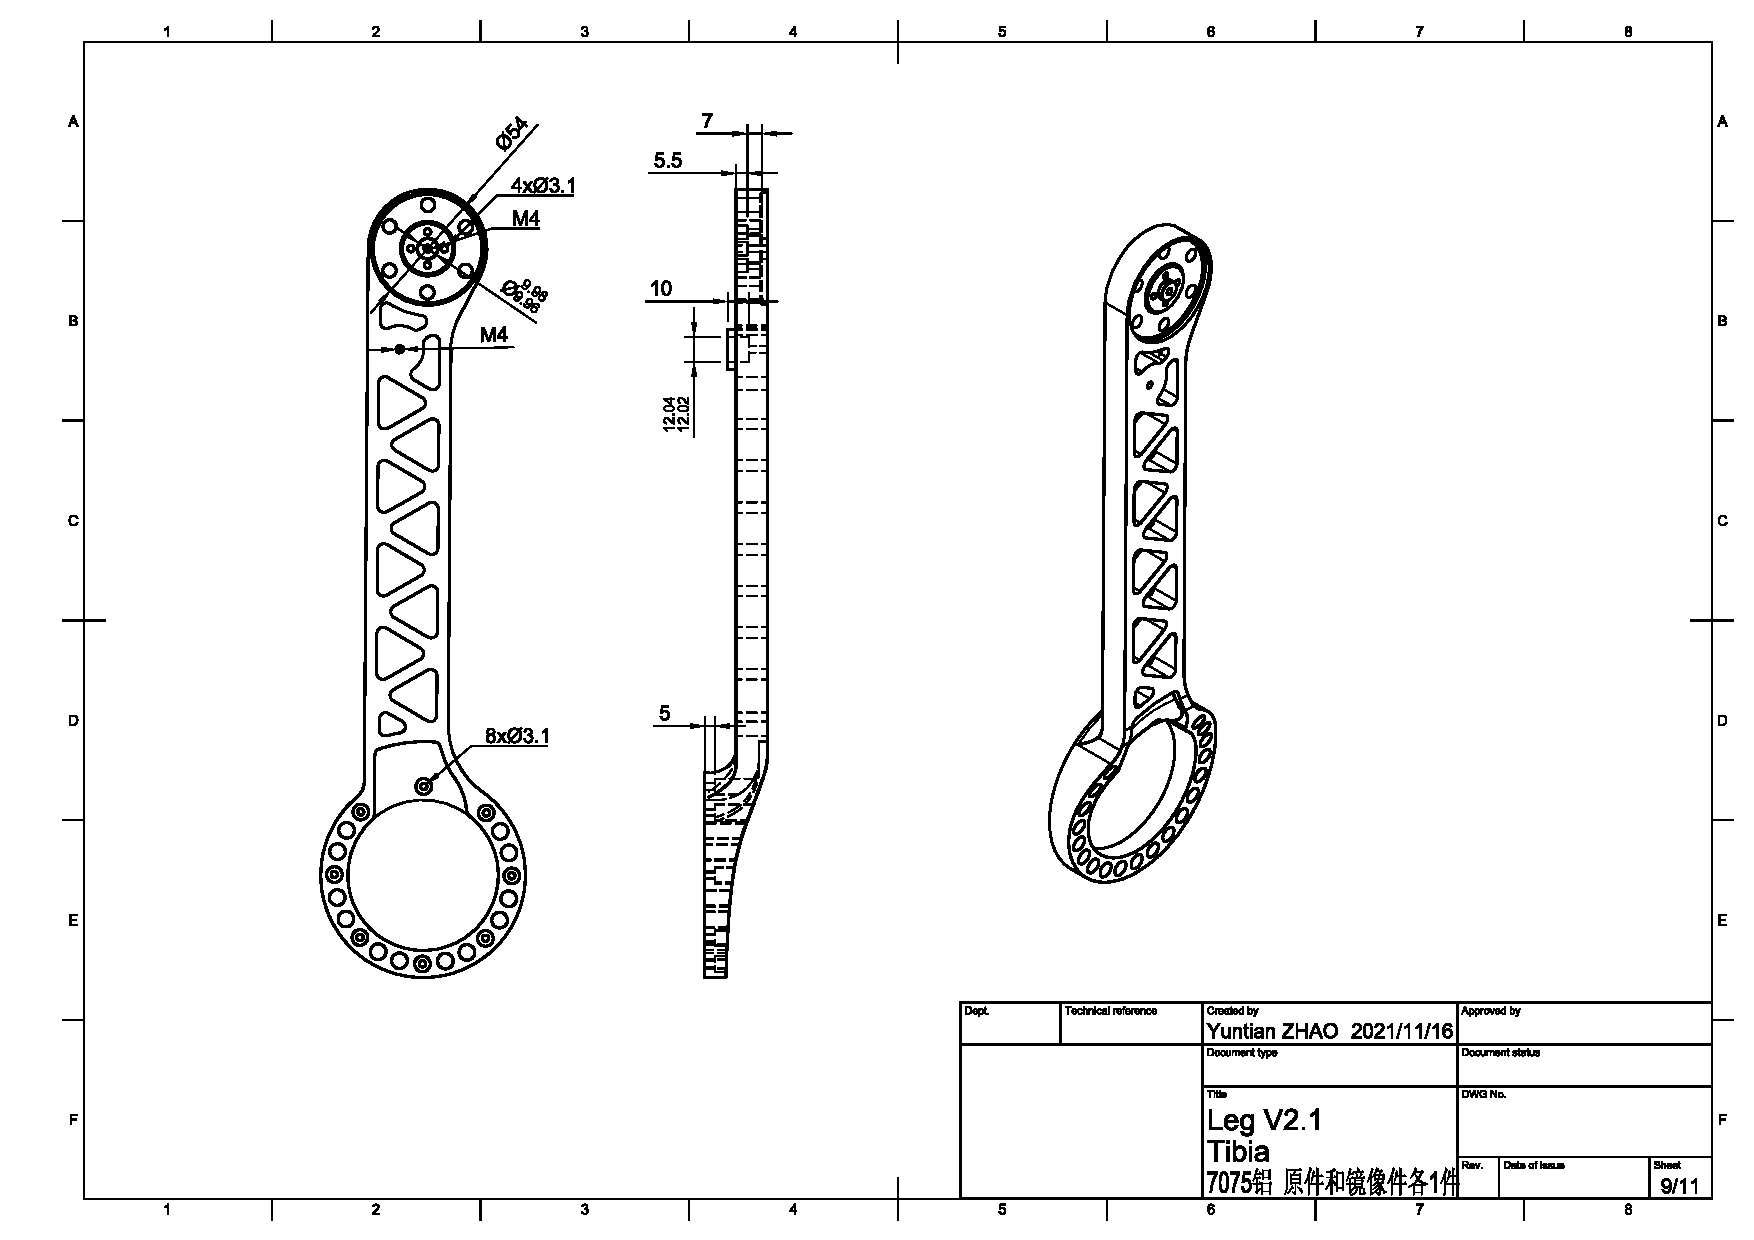
\includegraphics[width=1.4\linewidth, angle=90]{figures/appendix/dwg9.pdf}
   \vspace{6pt}
\end{figure}

\begin{figure}
  \centering
  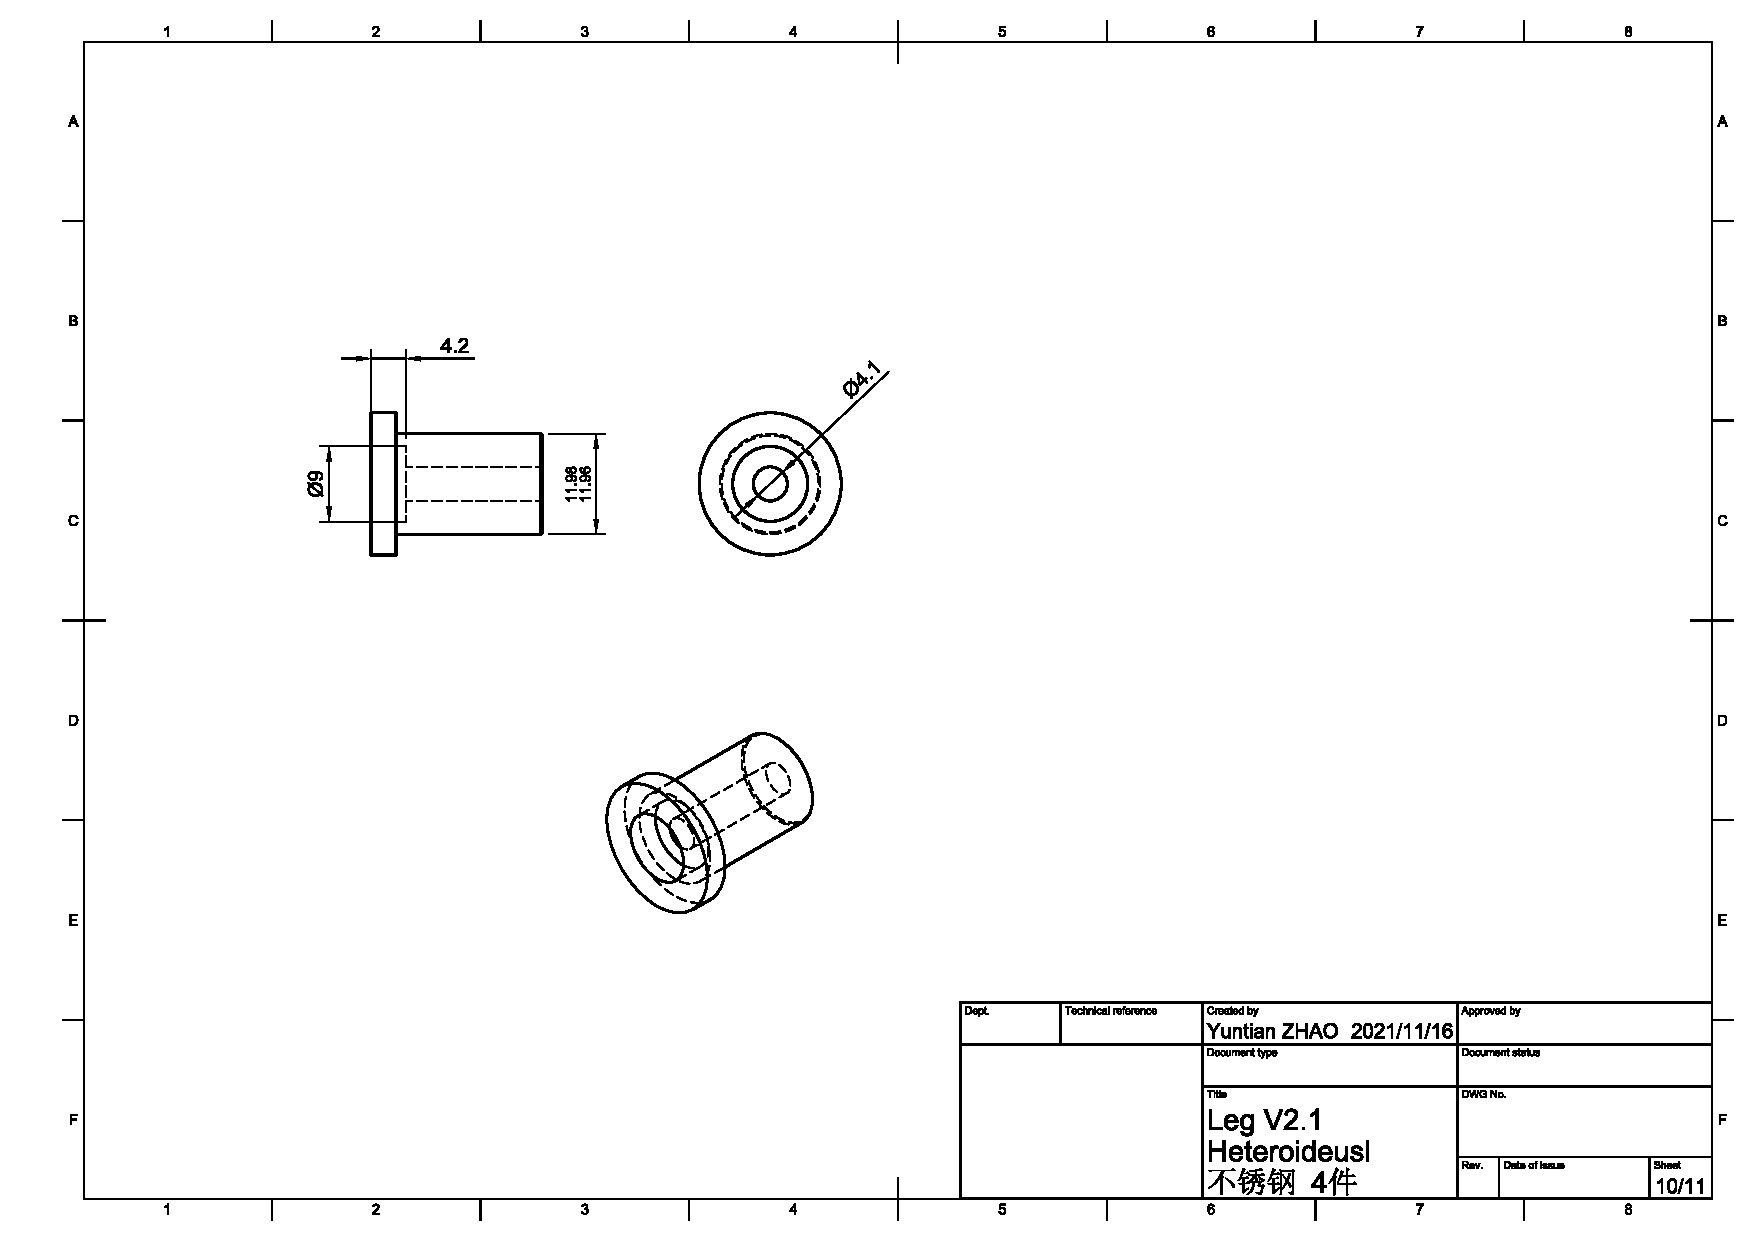
\includegraphics[width=1.4\linewidth, angle=90]{figures/appendix/dwg10.pdf}
   \vspace{6pt}
\end{figure}

\begin{figure}
  \centering
  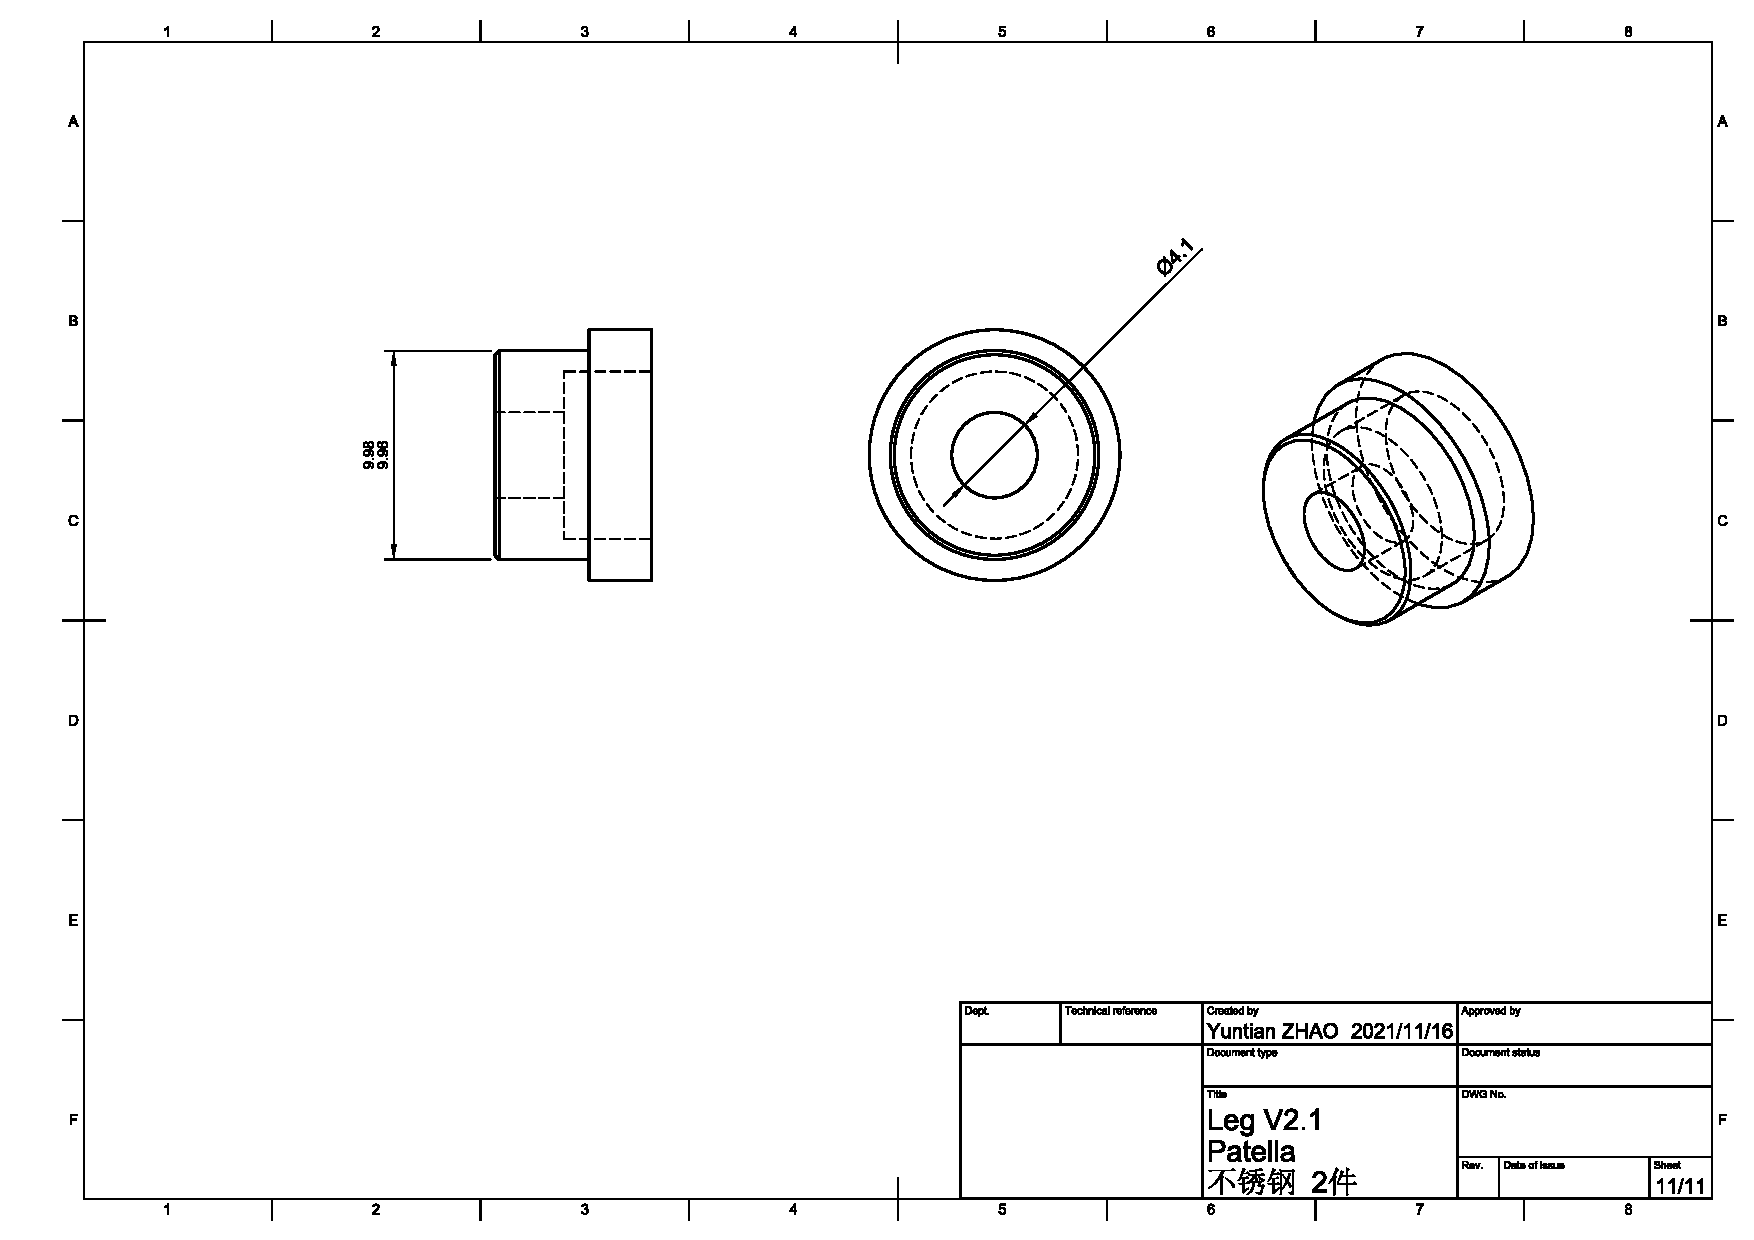
\includegraphics[width=1.4\linewidth, angle=90]{figures/appendix/dwg11.pdf}
   \vspace{6pt}
\end{figure}

\clearpage

\section*{部分3D打印件示意图}

\begin{figure}[h!]
  \centering
  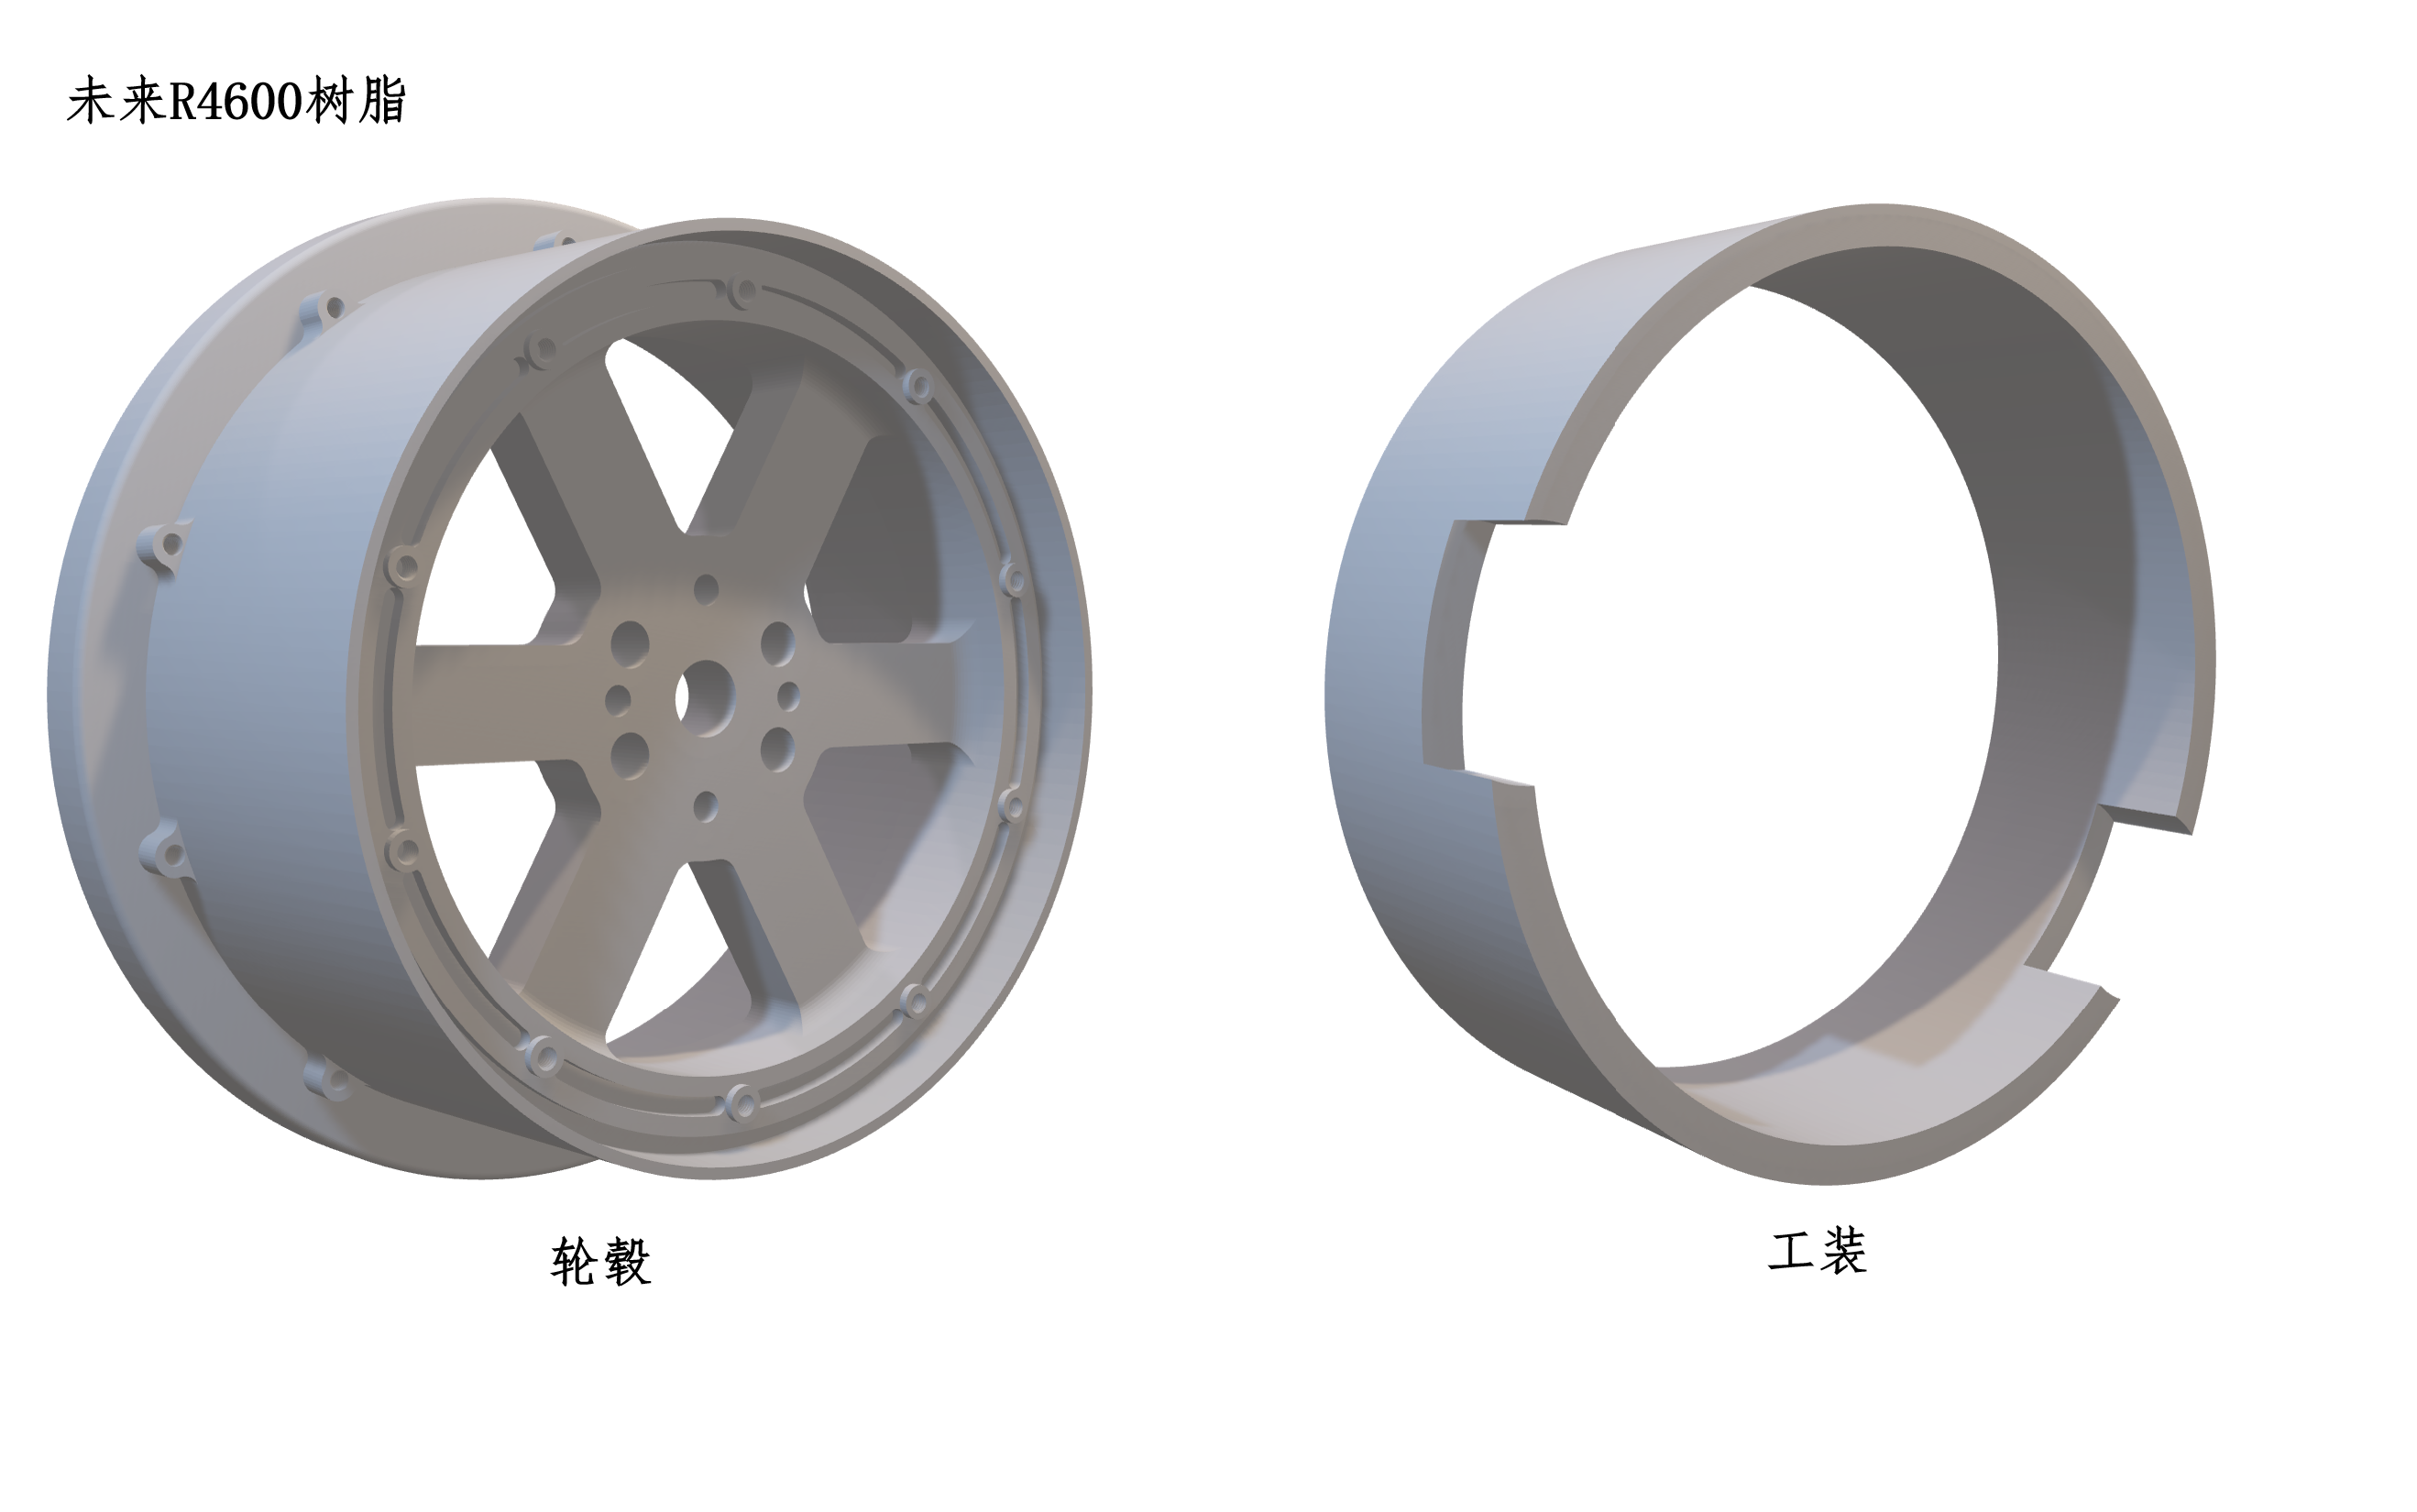
\includegraphics[width=1.4\linewidth, angle=90]{figures/appendix/3d1.png}
   \vspace{6pt}
\end{figure}

\begin{figure}
  \centering
  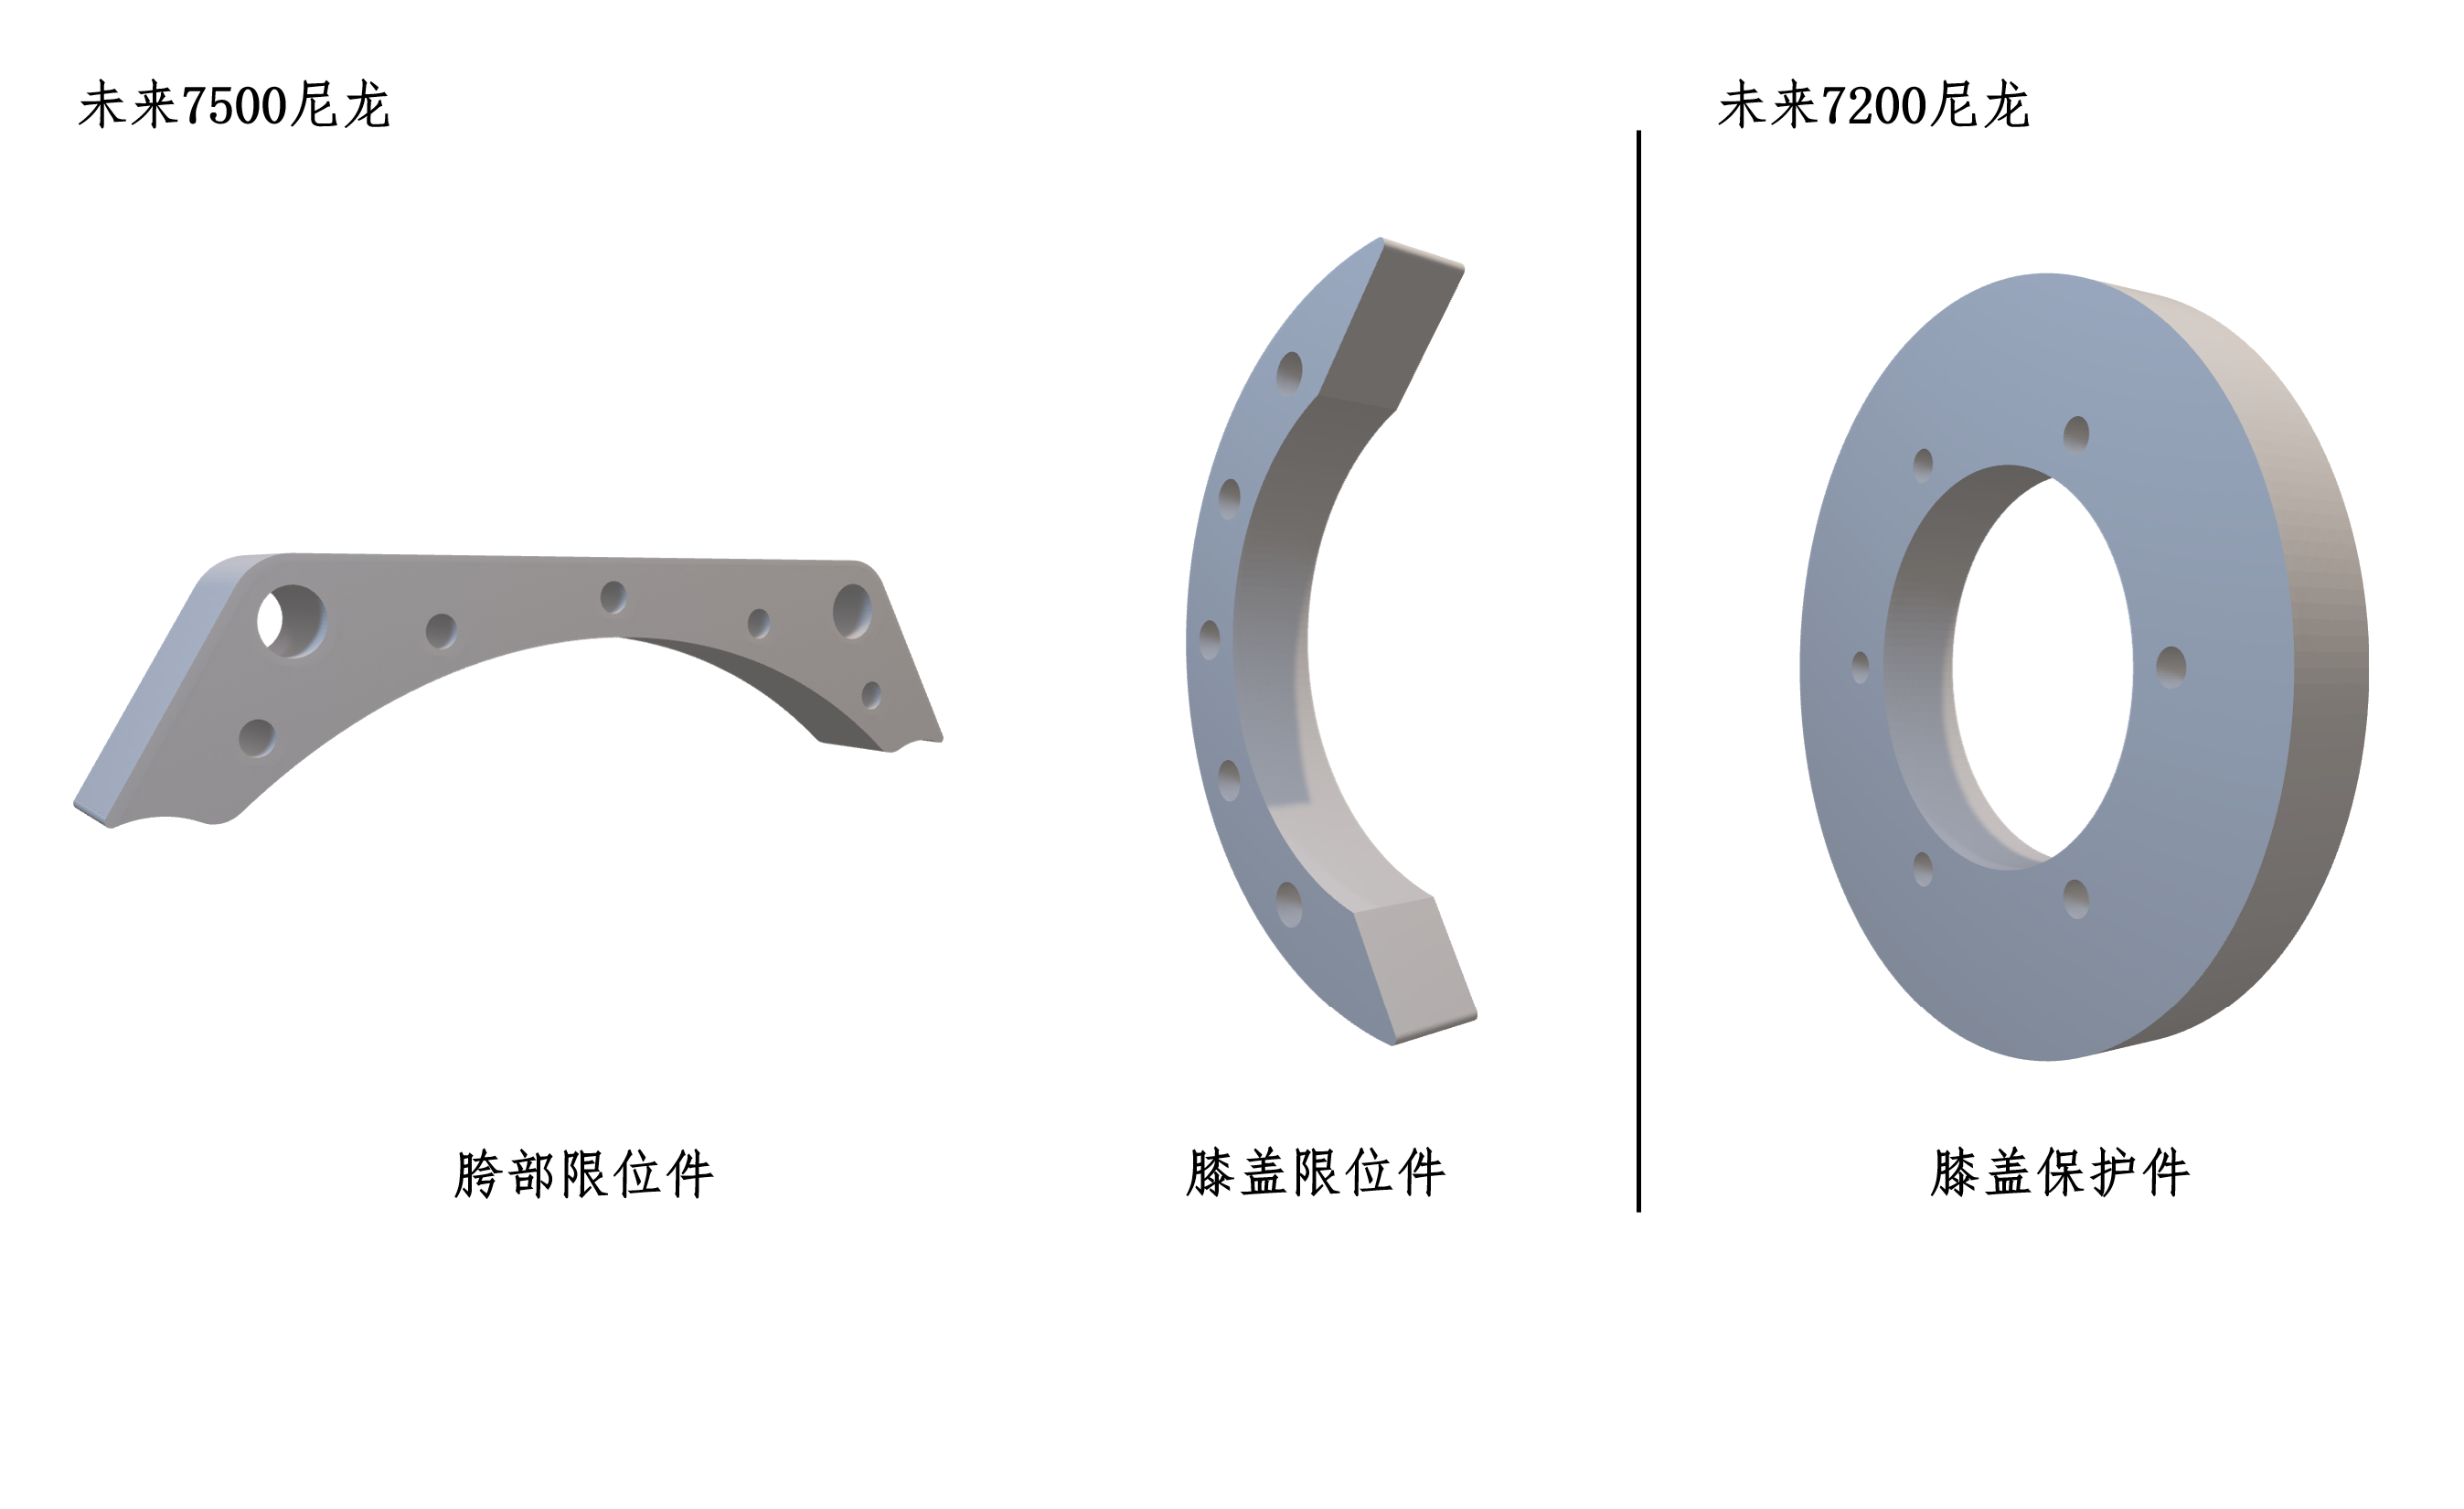
\includegraphics[width=1.4\linewidth, angle=90]{figures/appendix/3d2.png}
   \vspace{6pt}
\end{figure}

\begin{figure}
  \centering
  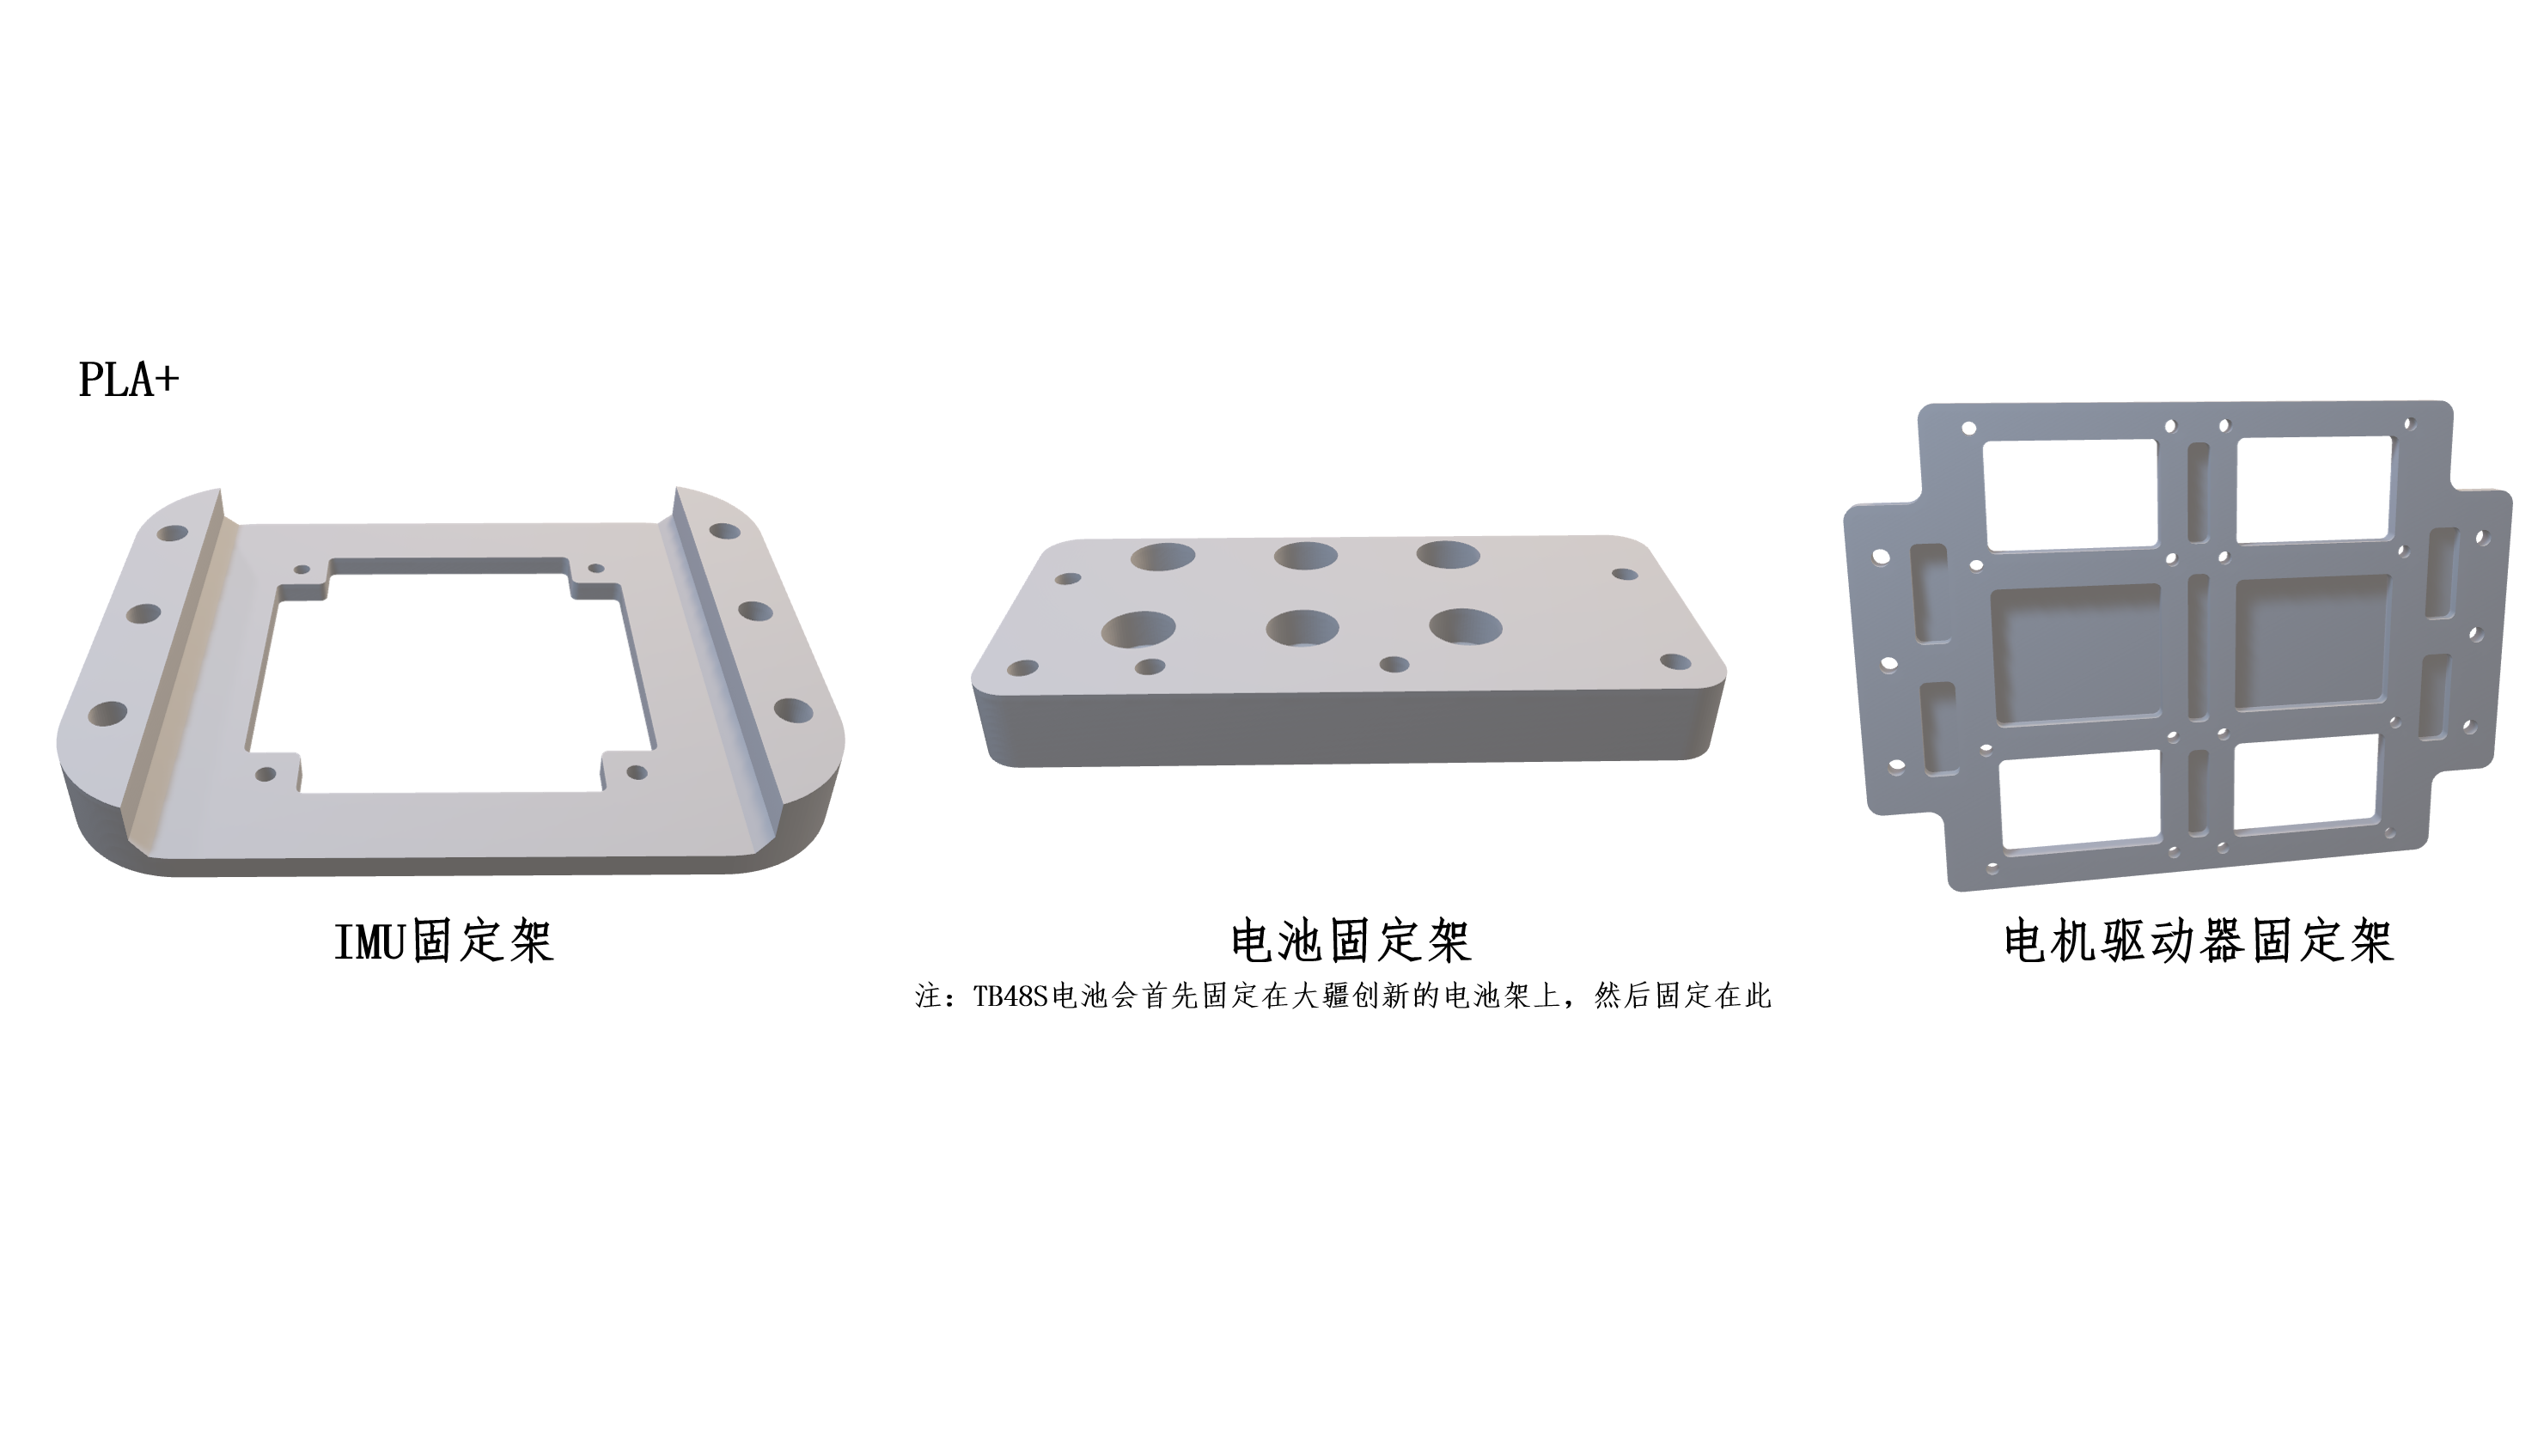
\includegraphics[width=1.4\linewidth, angle=90]{figures/appendix/3d3.png}
   \vspace{6pt}
\end{figure}

\clearpage

% \section*{机器人运动学及动力学参数}


% \clearpage
% \section*{状态机控制代码}


% \clearpage
% \section*{仿真及实验控制器参数}


% \clearpage